\documentclass[times]{qjrms4}
\usepackage[colorlinks,bookmarksopen,bookmarksnumbered,citecolor=red,urlcolor=red]{hyperref}
\usepackage{multirow} % for table using multiple rows
\usepackage{xr}
\usepackage{setspace}
\onehalfspacing
%\externaldocument{./Figures}
%\externaldocument{./Tables}
%\usepackage[pdftex]{graphicx}
%\usepackage{color}
%\usepackage{pdfpagediff}
%\layerPages{MainDocument.pdf}{../paper_final/MainDocument.pdf}


\begin{document}
\newcommand{\bcite}{\color{black}\citep}  

\begin{flushleft}
 {\bf{An Efficient Perturbed Parameter Scheme in the Lorenz system for Quantifying Model Uncertainty}} \\
 Gino Chen
\end{flushleft}


%\begin{abstract}
%	
The goal of this study is to develop a reliable and efficient perturbed parameter scheme
that is comparable to stochastic parameterizations.\ 
The Lorenz model is a simple testbed for numerical simulations.\
We have implemented a two time-scale Lorenz 63 (L63) model
to mimic the ocean-atmosphere coupled system, and 
a spatially-resolved convective-scale Lorenz 96 (L96) model 
coupled to the L63 atmospheric component.\
The full set of equations is defined as the ``truth".\
The spatially-resolved system will be parameterized 
by three different schemes: (i) deterministic, (ii) additive stochastic parameterization, and (iii) perturbed parameter.\
Perfect initial conditions are applied to investigate model error.\
By applying ``informative" probability distributions to the perturbed parameter scheme,
we have reduced systematic biases where previous implementations have failed to do so.\
Despite the fact that stochastic parameterizations are shown to resolve systematic errors,
they become computationally expensive in a GCM with 
more grid points to generate correlated stochasticity.\ 
The proposed scheme uses a stochastic spectral method,
Polynomial Chaos Expansion (PCE),
to approximate the exact ensemble states with minimum model simulations.\
Once built, PCE is implemented as a low cost sampling 
surrogate to generate large ensemble forecasts without actually integrating the model.\
The PCE-accelerated informative perturbed parameter scheme
generates competitive and reliable ensemble forecasts.\


%\end{abstract}

%\keywords{perturbed parameter, stochastic parameterization, 
%polynomial chaos, model uncertainty, ensemble forecast reliability, coupled predictability}

%\maketitle

\section{Introduction} 
	
The goal of this study is to develop a reliable and efficient perturbed parameter scheme
that is comparable to stochastic parameterizations.\ 
The Lorenz model is a simple testbed for numerical simulations.\
We have implemented a two time-scale Lorenz 63 (L63) model
to mimic the ocean-atmosphere coupled system, and 
a spatially-resolved convective-scale Lorenz 96 (L96) model 
coupled to the L63 atmospheric component.\
The full set of equations is defined as the ``truth".\
The spatially-resolved system will be parameterized 
by three different schemes: (i) deterministic, (ii) additive stochastic parameterization, and (iii) perturbed parameter.\
Perfect initial conditions are applied to investigate model error.\
By applying ``informative" probability distributions to the perturbed parameter scheme,
we have reduced systematic biases where previous implementations have failed to do so.\
Despite the fact that stochastic parameterizations are shown to resolve systematic errors,
they become computationally expensive in a GCM with 
more grid points to generate correlated stochasticity.\ 
The proposed scheme uses a stochastic spectral method,
Polynomial Chaos Expansion (PCE),
to approximate the exact ensemble states with minimum model simulations.\
Once built, PCE is implemented as a low cost sampling 
surrogate to generate large ensemble forecasts without actually integrating the model.\
The PCE-accelerated informative perturbed parameter scheme
generates competitive and reliable ensemble forecasts.\


\section{Experimental Setup}\label{sec:expsetup}
		%%%%%%%%%%%%%%%%%%%%%%%%%%%%%%%%%%%%%%	
	\subsection{The Coupled Lorenz System} 
	%%%%%%%%%%%%%%%%%%%%%%%%%%%%%%%%%%%%%%
		We use a two time-scale, coupled L63 model 
		{\citep{Lorenz63, Siqueira12}} where the fast component is analogous 
		to the atmosphere and the slow component is analogous to the ocean.\
		The atmospheric component is further coupled 
		to a small-scale spatially resolved system
		(high frequency small amplitude).\
		This spatially resolved system is composed of four
		identical dynamical equations of the convective-scale L96 model {\citep{Lorenz96}}
		each representing a spatial grid point with nonlinear 
		interaction with the neighbors.\
		The first and last grid point share the boundary.\
		The small-scale system could be seen
		as a convective process in the atmospheric component.\
		Therefore, a deterministic parameterization of the spatially resolved system
		is analogous to the bulk parameterization of the 
		subgrid-scale processes in the weather and climate models.\
		
		The atmospheric component:
		\begin{equation} \label{atmComp}
			\begin{aligned}
				&\frac{dX_1}{dt} = \sigma(X_2 - X_1) - a(Y_1 + k) - {\bold{U^*}} \\%{\dashbox{2.5}(20,20){U}}  \\
				&\frac{dX_2}{dt} = rX_1 - X_2 - X_1 X_3 + a(Y_2 + k) \\
				&\frac{dX_3}{dt} = X_1 X_2 - bX_3 + aY_3 \\
			\end{aligned}
		\end{equation}
		
		The oceanic component:
		\begin{equation} \label{ocnComp}
			\begin{aligned}
				&\frac{dY_1}{dt} = \tau \Big(\sigma(Y_2 - Y_1)\Big) - a(X_1 + k) \\
				&\frac{dY_2}{dt} = \tau(rY_1 - Y_2 - Y_1 Y_3) + a(X_2 + k) \\
				&\frac{dY_3}{dt} = \tau(Y_1 Y_2 - bY_3) + aX_3 \\
			\end{aligned}
		\end{equation}
		
		where $\bold{U^*} = \frac{a_z\tau_z}{s_z}\sum\limits_{i=1}^4 Z_i$ 
		(the term to be parameterized) 
		is associated to the spatially resolved system:
		\begin{equation} \label{subgridComp}
			\frac{dZ_i}{dt} = \tau_z \Big( -s_z Z_{i+1} (Z_{i+2} - Z_{i-1}) 
				- Z_i  + \frac{a_z}{s_z}X_1 \Big); \ \ i = 1,\dotsc,4 
		\end{equation}
		where $Z_0 = Z_4$, and $Z_5 = Z_1$.\ 
		The spatially resolved system represents the subgrid-scale processes
		after $\bold{U^*}$ is parameterized.\ 
%		(See Table {\ref{tab:ModParm}} for the parameter descriptions).\\


	%%%%%%%%%%%%%%%%%%%%%%%%%%%%%%%%%%%%%%	
	\subsection{Truth Model} 
	%%%%%%%%%%%%%%%%%%%%%%%%%%%%%%%%%%%%%%
%		ocean is 3.72 MTU, ocean is 2.79 MTU.\
	
		The true states are from the outputs of the entire set of 
		equations \eqref{atmComp}, \eqref{ocnComp} and \eqref{subgridComp}.\
		The equations are integrated by an adaptive 
		fourth-order Runge-Kutta (RK4) time-stepping scheme.
		A true time series of $1600$ Model Time Units (MTU) is generated
		(transient phase is removed) for the forecast models to compare with.\
		This study conducts a total of 300 forecast events (each of $25$ MTU) 
		with initial conditions selected from the $1600$ MTU truth time series at
		intervals of $5$ MTU where the atmospheric states generally lose correlation.\


		Following {\citet{Arnold13}}, we designed 
		two experiments by varying the time-scale 
		($\tau_z=2$ and $\tau_z=10$) for the spatially resolved system.\
		The \emph{error-doubling time}, approximately two atmospheric days by a GCM {\citep{Lorenz96}}, 
		in the atmospheric component is $1.47$ MTU for $\tau_z=2$, 
		and $1.10$ MTU for $\tau_z=10$.\ %averaged over 300 forecast events 
		Therefore the atmospheric component maximum forecast lead time for both experiments
		is selected to be $5$ MTU, which is in the range of $7$ to $10$ atmospheric days by a GCM.\
%		Figure {\ref{autocorr}} shows the time-lag autocorrelation coefficient of the true $r^k$ samples, 
%		with slow (fast) decay in the $\tau_z=2$ ($\tau_z=10$) experiment.\	
		The results using L96 as the coupled model {\citep{Wilks05, Arnold13}}
		stated that the slow evolving case ($\tau_z=2$ in our case) better represents a
		real atmospheric subgrid-scale process.\
		Whereas the subgrid-scale system at $\tau_z=10$ behaves like a white-noise process
		with less correlation between the time samples.\
		The contrasting subgrid-scale dynamics gives us the opportunity 
		to test the limits of our methodology.\

		
	%%%%%%%%%%%%%%%%%%%%%%%%%%%%%%%%%%%%%%	
	\subsection{Forecast Model} 
	%%%%%%%%%%%%%%%%%%%%%%%%%%%%%%%%%%%%%%
		The forecast model uses the atmosphere \eqref{atmComp} and ocean \eqref{ocnComp},
		and parameterizes $\bold{U^*}$ with $U_p$, thus 
		truncating the small-scale system \eqref{subgridComp}.\
%		The following sections will go through the three 
%		schemes of $U_p$ for the forecast model: 
		Three schemes of $U_p$ are compared for the forecast model:
		(i) deterministic, (ii) additive stochastic parameterization and
		(iii) the proposed perturbed parameter scheme.\


%\section{Deterministic Parameterization} \label{sec:schemesDet}
%			Figure {\ref{linearCurve}} (a) and (b) shows the discrete time samples of $(X_1^k, \bold{U^*}(X_1^k))$ (grey),
		where $k$ is the discrete time index.
		By fitting a cubic linear regression (black) through the cloud of time samples
		thus forms the deterministic parameterization
		\begin{equation}
			U_p = \bar{U} = \beta_0 + \beta_1 X_1 + \beta_2 X_1^2 + \beta_3 X_1^3.\
		\end{equation}
		The true residual is thus the difference between $\bold{U^*}$ and $\bar{U}$: 
		\begin{equation} \label{true_U}
			 r^k = \bold{U^*}(X_1^k) - \bar{U}(X_1^k).
		\end{equation}
		A total of $320,000$ $r^k$ samples are drawn from the $1600$ MTU time series every 
		$0.005$ MTU.\
		
		


%\section{Stochastic Parameterization} \label{sec:schemesStoch}
%			
		We have chosen to model $r^k$ as an additive stochastic parameter $e^k$
		based on the reliable forecast skill shown in \citet{Arnold13}.\
		Therefore, the additive stochastic parameterization for $\bold{U^*}$ is 
		\begin{equation} \label{stochParm}
			U_p = \bar{U} + e^k.\
		\end{equation}

%		despite a variety of stochastic parameterizations
%		(e.g., state dependent noise, multiplicative noise, etc).\
		
		The time series of $r^k$ in $\tau_z=2$ exhibits a high autocorrelation (Figure {\ref{autocorr}} (a)), 
		so it is reasonable to model $r^k$ as a $1^{st}$-order autoregressive process 
		(AR1) {\citep{Wilks11}}, where the discrete time samples of $e^k$ could be represented
		as a simple linear regression
		\begin{equation} \label{AR1}
			\begin{aligned}
			e^{k+1}
			& = \gamma e^k + \epsilon  \\
%			& = \gamma e^k + \sigma_\epsilon z \\
			& = \gamma e^k + (1-\gamma^2)^{1/2} \sigma_r z
			\end{aligned}
		\end{equation}
		where the predictand $e^{k+1}$ is updated by the predictor $e^k$ at the previous time sample,
		$\gamma$ is the 1-lag autocorrelation coefficient from the true residual, 
		and $\epsilon$ is the error of the simple regression.\
		Figure {\ref{linearCurve}} (c) and (d) shows a higher
		density near the deterministic curve and weakens away.\
		Therefore $\epsilon$ is modeled as a
		centered Gaussian process, 
		with a standard normal random variable $z$,
		and the standard deviation $\sigma_r$ of the true residuals.\
		The ensemble forecast of the additive stochastic parameterization 
		contains a total of 40 ensemble members for any event.\

		
		It is intuitive to represent the subgrid-scale 
		uncertainties with a time-varying $e^k$ since $r^k$ is constantly changing,
		but, there is no theoretical proof that a time-fixed $e$ is invalid.\
		This leads to the perturbed parameter scheme where 
		$e$ is fixed in time, which is no longer a stochastic process.\

		

%\section{The Proposed Efficient Perturbed Parameter Scheme} \label{sec:schemesPert}
%		
%		%%%%%%%%%%%%%%%%%%%%%%%%%%%%%%%%%%%%%%	
%		\subsection{Perturbed Parameter} 
%		%%%%%%%%%%%%%%%%%%%%%%%%%%%%%%%%%%%%%%	
		A perturbed parameter scheme treats $r^k$ as a time-invariant
		uncertain variable $e_s$ (a fixed value during model integration),
		\begin{equation} \label{perturbedParm}
			U_p = \bar{U} + e_s,			
		\end{equation}
		where the $k^{\text{th}}$ time index is dropped and replaced with
		the subscript $s$ representing ``stationarity".\
		The $e_s$ is a time-fixed perturbation on the regression parameter $\beta_0$ 
		(i.e., any perturbation to $\beta_0$ gives a constant 
		shift to $\bar{U}(X_1)$ along the $U$-axis).\
		Figure {\ref{blackPertCurve}} is the same as Figure {\ref{linearCurve}} (a) and (b), 
		where the black curves covering the cloud of true $\bold{U^*}$ (grey circles) show $\bar{U}$ perturbed by different values of $e_s$.\ 
		This allows us to control directly the distribution of $U_p(e_s)$ by assigning different distributions to $e_s$.
		A proper distribution of $U_p$ has the potential to capture the 
		true distribution of $\bold{U^*}$ and eventually impact the ensemble forecast skill
		(i.e., $X$'s and $Y$'s are both functions of $U_p$).\
		Therefore, this single perturbed parameter $e_s$ is used 
		in the proposed scheme (in contrast to using 
		all four parameters/regression coefficients in \citet{Arnold13}).\
		We designed both ``informative" and ``uninformative" 
		input distributions in Subsection \ref{subsec:dist_es}
		to emphasize the importance of reliable $e_s$ distributions.\
		In order to lower the cost when integrating over a large number of perturbed $e_s$,
		we build an emulator using a PCE, an analytical function of $e_s$.\ 
		The PCE-based surrogate is easy to evaluate and allows
		one to generate large ensemble states (e.g., $> 10^4$ ensemble members)
		without the need to integrate the actual model.\
		The PCE was initially developed by  {\citet{Wiener38}} 
		to address problems in statistical mechanics;
		it was applied in engineering mechanics to quantify
		uncertainties in stochastic Gaussian processes
		by {\citet{Ghanem90}}, and generalized to a wider range of stochastic processes by {\citet{Xiu02}}.

 

		
		
		%%%%%%%%%%%%%%%%%%%%%%%%%%%%%%%%%%%%%%%%%%
		\subsection{ PCE of a Perturbed State Variable} 
		%%%%%%%%%%%%%%%%%%%%%%%%%%%%%%%%%%%%%%%%%%	
		PCEs express the dependence of the model output variables
		on the input perturbation $e_s$ as a
		spectral series of the form {\citep{Maitre10}}:
		\begin{equation} \label{pce_compact}
			f(t,e_s) = \sum\limits_{ i=0 }^N \hat{f}_i(t)  P_i(\xi).
		\end{equation}
		where $f(t,e_s)$ is a model output variable (e.g., $X_1(t,e_s)$; separate independent PCEs can be
                constructed for any output quantity of interest),
		$\hat{f}_i(t)$ are the series coefficients,
		$P_i(\xi)$ are polynomial basis functions, 
                 $\xi$ is a standardized variable that maps the standard domain $-1\le\xi\le 1$ to the
		perturbation domain $r_{\min}\le e_s\le r_{\max}$
		\footnote{A linear mapping of the form $e_s = (r_{\max}-r_{\min}) \frac{\xi + 1}{2}+r_{\min}$ is sufficient. Here 
			$r_{\min}= \min_k r^k$ and $r_{\max} = \max_k r^k$ are the extrema of the true residual (equation \ref{true_U}).}.
		PCEs can be viewed as Fourier-like expansions in 
		the perturbed parameter and thus inherit their approximation properties; in particular PCEs
                converge spectrally fast when $f(t,e_s)$ varies smoothly with $e_s$.
		We suppress the time dependence of $f$ and $\hat{f}_i$ from now on to simplify notation.

			The basis functions are polynomials that
			are orthogonal with respect to an inner product defined by
			\begin{equation} \label{orthogonality}
				 \big< P_i,  P_j \big> 
				 = \int P_i(\xi) 
				 	P_j({\xi}) p(\xi) d\xi 
				 = \delta_{ij} \big< P_i^2 \big>
			\end{equation}
			where $\delta_{ij} = 1$ if $j=i$ and zero otherwise, and where $p(\xi)$ is a weight
			function\footnote{When the weight function coincides with the probability 
			distribution of $e_s$ the inner product can be interpreted as an expectation estimate of 
			$P_i P_j$; it is easy to show that the mean of $f$ w.r.t. $\xi$ is then simply the zeroth coefficient 
                        $\hat{f}_0$.}.
			This study uses Legendre polynomials for $P_i$, which are orthogonal 
			with respect to the uniformly distributed $\xi$ in the standardized domain $[-1 \ 1]$, 
			hence $p(\xi)=1/2$ is just constant over the domain.\
			The assumption of a uniformly distributed $\xi$ is not restrictive since, once the
			series coefficients are known, one could simply sample it with any 
			probability distribution desired.\ 
			A carefully selected distribution of $e_s$ will guarantee reliable forecasts
			since the sampling of $e_s$ affects directly the ensemble forecast state distributions.\
			This will be discussed in Subsection \ref{subsec:dist_es}.
			
			\emph{Spectral projection} can be used to obtain the coefficients $\hat{f}_{i}$, i.e.,
			one takes the inner product of equation \eqref{pce_compact} with each of the basis functions
			$P_j$ and invokes orthogonality to obtain: 
			\begin{equation} \label{PCoeff}
				\begin{aligned}
					\left< f, P_j \right>
						= \left<  \sum\limits_{i=0}^{N}
							\hat{f}_i P_i, P_j \right>
						= \hat{f}_i \left< P_i^2 \right>,
				\end{aligned}
			\mbox{ or }
				\hat{f}_i = \frac{\left< f, P_i \right>}
					{\left< P_i^2 \right>}.
			\end{equation}
			Since $f$ is not an analytical function, we use quadrature 
			(i.e., numerical integration) to approximate the numerator in \eqref{PCoeff}:
			\begin{equation}	\label{1DQ}
				\left< f, P_i \right> = \int_{-1}^1 f P_i p(\xi) d\xi \approx 
				\sum\limits_{q = 1}^{n} w_q f(t,\xi_q) P_i(\xi_q)
			\end{equation}
			$\xi_q$ are the quadrature points,
			and $w_q$ are the associated quadrature weights
			\footnote{ We have employed 
			Clenshaw-Curtis nested quadrature rule {\citep{Clenshaw60}} whose accuracy can be
			improved by increasing the number of quadrature points $n$; an $n$ point Clenshaw-Curtis quadrature would be
			exact if $(fP_ip)$ is a polynomial of degree $(n-1)$. }.
                        The evaluation of the series coefficients requires thus an ensemble of model runs to obtain
			$f(\xi_q)$ (the ensemble members correspond to setting the perturbed parameter to its value at the quadrature
			point and running the model); no code modification is needed.
			The black lines in Figure {\ref{blackPertCurve}} show 
			$U_p$ evaluated at the quadrature points, namely $e_s(\xi_q)$. 
			Equation \eqref{PCoeff} becomes
			\begin{equation} \label{PCoeff_num}
				\hat{f}_i = \frac{\sum_{i=1}^n  P_i(\xi_q) w_q f(\xi_q)}
					{\left< P_i^2 \right>}.\
			\end{equation}		
			The combination of equations \eqref{PCoeff_num} and \eqref{pce_compact}
			completes the PCE surrogate model for the perturbed forecast state variable.\
			

			As mentioned earlier, $\tau_z=2$ may be closer to a real
			atmosphere-ocean coupled system, and the atmospheric variables exhibit a relatively smooth
			variations with $e_s$. A relatively short spectral series is then expected to represent
			accurately this dependency. 
			The $\tau=10$ experiment, on the
			other hand, exhibits large jump discontinuities (and ensuing Gibbs oscillations) 
			whose number increases with longer lead time ($\ge 10$MTU).
			The discontinuities hinder the convergence rate of the PCE and a longer series is
			then needed to represent the functional relationship between the state variables and the perturbation parameter.
			The $\tau=10$ experiment required a $64^{\text{th}}$ degree polynomial and hence an ensemble size of $129$ is needed for the 
			quadrature. We use a similar sized ensemble for the $\tau=2$ experiment even though a $16^{\text{th}}$ degree polynomial
			(and $33$ ensemble members) would have been sufficient.
			The observed jump phenomena will be discussed in Subsection \ref{subsec:num_cons}.\
%			\footnote{ $33$ ($129$) quadrature points correspond to using $6^{th}$ ($8^{th}$) 
%			level Clenshaw-Curtis quadrature rule.\ }
%			Runge's phenomenon could be 
%			alleviated by dividing the uncertainty domain into local PCE 
%			approximation of piece-wise continuous function 
%			using less model runs and more accurately capturing the solution {\citep{Wan05}}.\
%			(with $8-th$ level Clenshaw-Curtis quadrature rule)
			
			Once built, PCE of a forecast state variable allows one to test any distribution of 
			$e_s$ without actually integrating the model.\
%			(other than the simulations on the quadrature points required to build the PC coefficients).\
			The perturbed parameter scheme is thus performed by sampling 
			the $e_s$ from the PCE with a proper distribution to give 
			an ensemble state distribution that generates reliable forecast.\ 


		%%%%%%%%%%%%%%%%%%%%%%%%%%%%%%%%%%%%%%			
		\subsection{Distributions of $e_s$} \label{subsec:dist_es}
		%%%%%%%%%%%%%%%%%%%%%%%%%%%%%%%%%%%%%%
			In this study, $e_s$ is defined to be ``informative" when the samples 
			contain the true residuals $r^k$, and ``uninformative" when they are sampled from an 
			arbitrarily assigned distribution.

			In this study we assigned three distributions to $e_s$:
			$e_{\text{unif}}$, $e_{\text{clim}}$ and $e_{\text{AR1}}$.\
			The $e_{\text{unif}}$ distribution is uninformative and its samples are randomly 
			generated from a uniform distribution,
			whereas $e_{\text{clim}}$ and $e_{\text{AR1}}$ contain informative samples of $r^k$.\
			The $e_{\text{clim}}$ distribution was designed 
			to verify the existence of a single climatological distribution of $e_s$ for all forecast events; $e_{\text{clim}}$ is
			expected to be the most informative
			since it is based on the entire time series (1,600 MTU) of true $r^k$ samples.\
			Figure {\ref{hist_r}} shows the distribution of the $e_{\text{clim}}$
			using all $320,000$ $r^k$ time samples.\
			The $e_{\text{AR1}}$ distribution is based on
			the collection of all $e^k$ samples generated by the 
			40 ensemble members (25 MTU each) of the AR1-process for any forecast event.\
			The $e_{\text{AR1}}$ remains informative
			since the AR1 process begins with a single true $r^k$ sample.
			A total of 300 distributions (corresponding to 300 forecast events) are constructed for $e_{\text{AR1}}$
			to check whether using the samples from the stochastic parameterization 
			and modifying them into a stationary
			distribution could achieve equivalent forecast skill. \
%			Since $e_{\text{AR1}}$ has a memory from the initial truth $r^k$, it
%			is expected to show superiority	over the uninformative $e_{\text{unif}}$.\
%			The samples of all three distributions of 
%			$e_{\text{unif}}$, $e_{\text{clim}}$, and $e_{\text{AR1}}$
%			are evaluated by the same PCE at any given lead time for the ensemble state variables.\ 
%			Three separate distributions of the forecast states 
%			will be generated accordingly.\
			
		%%%%%%%%%%%%%%%%%%%%%%%%%%%%%%%%%
		\subsection{Summary of the Proposed Scheme} 
		%%%%%%%%%%%%%%%%%%%%%%%%%%%%%%%%%
			\begin{itemize}
				\item Obtain the spectral coefficients, $\hat{f}_i$, following the quadrature rule.\
				\item Construct the PCE approximation, $f(t,e_s)$, 
					of the forecast state variables $X$'s and $Y$'s.\
				\item Obtain the ensemble states of all three input distributions of 
					$e_s$ by individually sampling the PCE at the given lead times.\		
			\end{itemize}
			
			
		%%%%%%%%%%%%%%%%%%%%%%%%%%%%%%%%%
		\subsection {Numerical Consistency of PCEs} \label{subsec:num_cons}	
		%%%%%%%%%%%%%%%%%%%%%%%%%%%%%%%%%
			The Root Mean Squared Difference (RMSD) is applied to measure
			the accuracy of PCE in capturing the exact model solutions.\
			The exact solutions are generated by directly integrating the 
			forecast model from a uniformly sampled $e_s$.\ 
			The same collection of samples are then evaluated by PCE.\
			The RMSD is then calculated between the exact and PCE-generated solutions.\


			Figure {\ref{rmseQpt}} shows the time series of RMSD averaged over 300 events.\ 
			It also shows how well the PCE captures 
			the exact solution as the model evolves, and how fast
			it diverges from the exact solution given different $\tau_z$.\
			The PCE deteriorates, and its corresponding RMSD grows, as bifurcations in the
                        states, amplified by nonlinear dynamics, create 
			jump discontinuities.
			These discontinuities reflect the relative predictability of the atmosphereic and oceanic component.\
			The bigger RMSD growth rate in the atmospheric component 
			is analogous to the growth rate of a realistic coupled system, where
			the atmosphere generally loses predictability faster than the ocean.\
			The atmospheric RMSD (grey) in $\tau_z=10$ (bottom) 
			saturates sooner than that in $\tau_z=2$ (top) because of 
                        % which indicates that the PCE approximation deteriorated by 
                        the increasing
			large jump discontinuities for the $\tau_z=10$ case.\
			The ocean (black) shows slower RMSD saturation because it suffers
			fewer bifurcations in the ensemble states than the atmosphere.

%			This figure is also a reference to restrict the maximum forecast lead time
%			at $5$ MTU for atmospheric component and $25$ MTU for oceanic component.\


			The qualitative differences in PCE-approximated solutions and exact solutions
			are shown in Figure {\ref{respSfc1}} ($\tau_z=2$) and Figure {\ref{respSfc2}} ($\tau_z=10$).\
			The two figures show the forecast state as a function of the 
			input perturbation $e_{\text{unif}}$ at different forecast lead times (shown above each panel)
			from the view of a single event.\
			They show how different time-scale
			of the subgrid-scale system impacts PCE approximation.\ 
			The $\tau_z=10$ case exhibits fast evolving states and multiple
			big jump discontinuities, which lead to slower convergence for the PCE,
			especially in the atmospheric component.\
			Although the ocean component 
			bifurcates multiple times in both experiments,
			the overall state spread remained in a relatively 
			narrow range (with small amplitude jumps), and
			the errors in the PCE-generated ocean ensemble remained
			small.\


			Figure {\ref{pdf1}} and Figure {\ref{pdf2}} show 
			the evolution of the state p.d.f of the exact ensemble versus PCE-generated ensemble
			\footnote{Apply kernel density estimation following {\citet{Botev10}} } 
			with respect to Figure {\ref{respSfc1}} and Figure {\ref{respSfc2}}.\
			The features of the p.d.f. shown in this event are ubiquitous in other forecast events.\
			The distributions of the atmospheric states (top panels) 
			at $\tau_z=10$ (Figure {\ref{pdf2}}) spread along 
			a wider range with larger variances
			in all lead times and constantly changing shapes (non-Gaussian).\
			Therefore the impact of input distributions of $e_s$ on the ensemble distributions
			indicate the necessity of applying informative $e_{\text{clim}}$ or $e_{\text{AR1}}$).\
			The largely bifurcated nature in $\tau_z=10$ hinders the accuracy of
			PCE on approximating the exact states at longer lead time
			(e.g., the bottom rightmost panel in Figure {\ref{pdf2}}).\
						
 

			

%\section{Forecast Consistency} \label{sec:statConsistency}
%	\input{./ForecastConsistency}	
\section{Results} \label{sec:skills}
	
	The forecast skill of the ensemble schemes is evaluated by three scores,
	Reliability (REL), Ignorance Skill Score (IGNSS) and Ranked Probability Skill Score (RPSS).\
%	REL (a component of Brier Score for dichotomous events) 
%	measures whether the model is well-calibrated.\
%	IGNSS is a measure of dispersion of the ensemble, it assigns
%	penalty to underdispersed ensembles that cause systematic errors.\
%	RPSS evaluates a multi-category event,
%	it assigns penalty to the ensemble members that are further away from the category of occurrence 
%	(i.e., penalizes with a distance measure).\
%	For RPSS and IGNSS, the forecast states are divided into $10$ 
%	categories, which are the deciles of the climatological distribution.\


	
	% Discuss the overall PCE method doing
	Figure {\ref{scoreTau2}} ($\tau_z=2$) and Figure {\ref{scoreTau10}} ($\tau_z=10$) 
	show the time evolution of three scores 
	RPSS (top), IGNSS (middle) and REL (bottom) generated by the schemes:
	(I) Uninformative perturbed parameter ($e_{\text{unif}}$),
	(II) Informative perturbed parameter ($e_{\text{clim}}$, $e_{\text{AR1}}$), 
	(III) Additive stochastic parameterization (\emph{Stoch}), 
	(IIII) Deterministic parameterization (\emph{Det}). 
	The PCE for the perturbed parameter scheme in the two figures is approximated by $64^{\text{th}}$ degree polynomial.\
	As expected, without a probabilistic feature, \emph{Det} performed poorly over all scores.\
	Therefore, we only compare the \emph{Stoch}, and the perturbed parameter scheme using  
	$e_{\text{clim}}$, $e_{\text{AR1}}$ and $e_{\text{unif}}$ in the following.\


	Results in Figure {\ref{scoreTau2}} and Figure {\ref{scoreTau10}}
	show consistent and nearly identical scores by $e_{\text{clim}}$ and $e_{\text{AR1}}$.\
	This supports the hypothesis of applying informative distributions, regardless of the
	highly bifurcated the states in $\tau_z=10$, for the perturbed parameter scheme.

	At $\tau_z=10$, the uninformative $e_{\text{unif}}$ performs poorly in Figure {\ref{scoreTau10}} (a) and (c).\
	The failure is attributed to the wide ensemble spread (caused by strong bifurcations) at $\tau_z=10$.\
	Suppose the wide-spread case ($\tau_z=10$) and 
	the small-spread case ($\tau_z=2$) both forecast low density 
	at the category of occurrence by using $e_{\text{unif}}$.\
	The small-spread case will remain reliable with the entire ensemble
	contained in (or in close proximity to) the category of occurrence.\
	Whereas the wide-spread case using the uninformative input may have its highest density 
	erroneously far from the category of occurrence, resulting in a penalty in RPSS.\
	This explains why it is necessary to apply informative $e_s$, 
	especially when forecasting the wide-spread cases.\ 

%	At $\tau_z=2$, \emph{Stoch} underperformed in Figure {\ref{scoreTau2}} (c), (d) and (e)
%	with contrasting results in $\tau_z=10$ (Figure {\ref{scoreTau10}}),
%	which are attributed to two possible explanations: 
%	1) At $\tau_z=2$ ($\tau_z=10$), the slow (fast) varying, less (more) white noise like, subgrid-scale dynamics
%	is harder (easier) to be modeled by a stochastic process, and
%	2) the Gaussian stochastic term $\epsilon$ in equation \eqref{AR1} may 
%	not (may) represent a non-Gaussian (Gaussian-like) true residual in Figure {\ref{hist_r}} (a) (in Figure {\ref{hist_r}} (b)).\

%	In order to demonstrate the overall cost reduction by the PCE, 
%	we show a low order ($16^{\text{th}}$ degree polynomial) PCE forecast skill in Figure {\ref{scoreTau2_lev6}}
%	by keeping other schemes unchanged as in Figure {\ref{scoreTau2}}.\
%	The overall performance of the two informative $e_{\text{clim}}$ and $e_{\text{AR1}}$ 
%	are comparable to \emph{Stoch} by using significantly less simulations.\
%	This demonstrates that with a relatively smooth state ($\tau_z=2$), PCE could substantially reduce the computational cost.\
%	The weaker IGNSS (d) and REL (f) at longer lead time ($\ge 10$ MTU) in the ocean component
%	is caused by low order PCE converging slower when the jump discontinuities begin to increase.\
%	Despite the weakness, IGNSS and REL (Figure {\ref{scoreTau2_lev6}} (c) and (e)) 
%	by $e_{\text{clim}}$ and $e_{\text{AR1}}$ remain better than \emph{Stoch} 
%	in the atmosphere with shorter lead times ($\le 5$ MTU).

	
		
\section{Concluding Remarks and Future Work}
	
	We have implemented a coupled ocean-atmosphere system (L63) with a subgrid-scale 
	system (L96) in the atmospheric component.\
	The major result is to generate reliable forecasts
	by the proposed perturbed parameter scheme through
	the employment of informative input distributions.
	The informative perturbed parameter scheme especially outperformed an additive stochastic 
	parameterization in a more realistic subgrid-scale system ($\tau_z=2$).
	The low cost PCE surrogate guarantees unbiased statistics at large ensemble size,	
	and effectively delivers the ensemble distributions without the need to integrate the actual forecast model.\ 
	The numerical integration (i.e., quadrature) to build the PCE treats the 
	model as a black box, which is an advantage for operational forecasts using complex GCMs.\
	

%	Due to the strong bifurcation at longer lead times in a fast varying system ($\tau_z=10$), 
%	the estimation of exact states requires higher order PCE.\
%	The multiple large jump discontinuities may not be observed in a realistic dynamical system.\
%	Thus the proposition of PCE being efficient is not violated 
%	when given a relatively smooth and realistic experiment ($\tau_z=2$),
	%or forecasts created at a shorter lead time 
	%($<10$ MTU, or approximately less than $14$ atmospheric days).\
	
	The forecast skill of using just a single perturbed parameter
	for the PCE-accelerated informative perturbed parameter scheme
	is surprisingly competitive with the additive stochastic parameterization.\ 
	The challenge is to apply this to a realistic model with more parameters,
	where our forecast framework is developed to test multiple perturbed parameters effectively.\



%\appendix 
%\section{Example of the Galerkin Method} \label{sec:galerkin}
%	\input{./Appendix}
\begin{thebibliography}{99}

%\bibitem[Alexanderian et al.~(2012)]{Alex12}
%Alexanderian A, Winokur J, Sraj I, Srinivasan A, Iskandarani M, Thacker WC, Knio OM. 2012
%\emph{Global sensitivity analysis in an ocean general circulation model: a sparse spectral projection approach.},
%Computational Geosciences, 16(3):757-778 

\bibitem[Arnold et al. (2013)]{Arnold13}
Arnold HM, Moroz IM and Palmer TN. 2013
\emph{Stochastic Parametrizations and Model Uncertainty in the Lorenz'96 System.},
Philos. Trans. A Math. Phys. Eng. Sci., 371

%\bibitem[Berner et al. (2009)]{Berner09}
%Berner J, Shutts GJ, Leutbecher M and Palmer TN. 2009
%\emph{A Spectral Stochastic Kinetic Energy Backscatter Scheme and Its Impact on Flow-Dependent Predictability in the ECMWF Ensemble Prediction System.},
%J. Atmospheric Sci., 66: 603-626 

%\bibitem[Botev et al. (2010)]{Botev10}
%Botev ZI, Grotowski JF and Kroese DP. 2010
%\emph{Kernel Density Estimation Via Diffusion.},
%Annals of Statistics, 38:2916-2957

%\bibitem[Bowler et al. (2008)]{Bowler08}
%Bowler NE, Arribas A, Mylne KR, Robertson KB and Beare SE. 2008
%\emph{The MOGREPS short-range ensemble prediction system.},
%Q. J. R. Meteorol. Soc., 134:703-722 

%\bibitem[Bowler et al. (2009)]{Bowler09}
%Bowler NE, Arribas A, Beare SE, Mylne KR and Shutts GJ. 2009
%\emph{The local ETKF and SKEB: Upgrades to the MOGREPS short-range ensemble prediction system.},
%Q. J. R. Meteorol. Soc., 135:767�776 

%\bibitem[Buizza et al. (2005)]{Buizza05}
%Buizza R, Houtekamer PL, Toth Z, Pellerin G, Wei Mand Zhu Y. 2005
%\emph{A Comparison of the ECMWF, MSC, and NCEP Global Ensemble Prediction Systems.},
%Monthly Weather Review, 133:1076-1098

%\bibitem[Buizza et al. (1999)]{Buizza99}
%Buizza R, Miller M and Palmer TN. 1999
%\emph{Stochastic Representation of Model Uncertainties in the ECMWF Ensemble Prediction System.},
%Q. J. R. Meteorol. Soc., 125: 2887-2908

%\bibitem[Clenshaw and Curtis (1960)]{Clenshaw60}
%Clenshaw CW and Curtis AR. 1960
%\emph{A Method for Numerical Integration on an Automatic Computer.},
%Numerische Mathematik, 2:197-205 

%\bibitem[Conrad and Marzouk (2012)]{Conrad12}
%Conrad PR and Marzouk YM. 2012
%\emph{Adaptive Smolyak pseudospectral approximation.},
%CoRR abs/1209.1406
%
%\bibitem[Constantine et al (2012)]{Constantine12}
%Constantine PG, Eldred MS, Phipps ET. 2012
%\emph{Sparse Pseudospectral Approximation Method.},
%Comput. Methods Appl. Mech. Engrg., 229-232:1-12
%
%
%\bibitem[Gerstner and Griebel (2003)]{Gerstner03}
%Gerstner T and Griebel M. 2003
%\emph{Dimension Adaptive Tensor Product Quadrature.},
% Journal Computing archive, Vol. 71(1):65-87
% 
%\bibitem[Ghanem and Spanos (1990)]{Ghanem90}
%Ghanem R and Spanos PD. 1990
%\emph{Polynomial Chaos in Stochastic Finite Elements.},
%Journal of Applied Mechanics, 57:197-202
%
%\bibitem[Hosder et al. (2006)]{Hosder06}
%Hosder S, Walters RW and Perez R. 2006
%\emph{A Non-Intrusive Polynomial Chaos Method For
%Uncertainty Propagation in CFD Simulations.},
%44th AIAA Sciences Meeting and Exhibit
%
%\bibitem[Houtekamer et al. (1996)]{Houtekamer96}
%Houtekamer PL, Lefaivre L, Derome J, Ritchie H and Mitchell HL. 1996
%\emph{A System Simulation Approach to Ensemble Prediction.},
%Monthly Weather Review, 124: 1225-1241
%
%\bibitem[Kirtman et al. (2014)]{Kirtman14}
%Kirtman BP and Coauthors. 2014
%\emph{The North American Multimodel Ensemble: Phase-1 
%Seasonal-to-Interannual Prediction; Phase-2 toward Developing Intraseasonal Prediction.},
%Bull. Amer. Meteor. Soc., 95: 585�601
%
%\bibitem[Leutbecher and Palmer (2008)]{Leutbecher08}
%Leutbecher M and Palmer TN. 2008
%\emph{Ensemble Forecasting.},
%J. Computational Physics, 227: 3515-3539
%
\bibitem[Lorenz (2006)]{Lorenz96}
Lorenz EN. 2006
\emph{Predictability - A Problem Partly Solved.},
Cambridge University Press, 40-58
%
\bibitem[Lorenz (1963)]{Lorenz63}
Lorenz EN. 1963
\emph{Deterministic Nonperiodic Flow.},
Journal Atmospheric Sciences, 20:130-141
%
%\bibitem[Lucor et al. (2001)]{Lucor01}
%Lucor D, Xiu D and Karniadakis G. 2001
%\emph{Spectral Representation of Uncertainty in Simulations: Algorithms and Application.}, 
%ICOSAHOM-01, Uppsala Sweden
%
%
%\bibitem[Palmer et al. (2009)]{Palmer09}
%Palmer TN, Buizza R, Doblas-Reyes F, Jung T, Leutbecher M,  Shutts GJ,  Steinheimer M and  Weisheimer A. 2009 
%\emph{Stochastic Parametrization and Model Uncertainty.},
%ECMWF Technical Memorandum, 598
%
%\bibitem[Palmer (2001)]{Palmer01}
%Palmer TN. 2001
%\emph{A Nonlinear Dynamical Perspective on Model Error- A Proposal for 
%Non-local  Stochastic-dynamic Parametrization in Weather and Climate Prediction Models.},
%Q. J. R. Meteorol. Soc., 127:279-304
%
%\bibitem[Pennell and Reichler (2011)]{Pennell11}
%Pennell C and Reichler T. 2011
%\emph{On the effective number of climate models.},
%J. Clim., 22:2358�2367
%
%\bibitem[Le Maitre and Knio (2010)]{Maitre10}
%Le Maitre OP and OM Knio. 2010
%\emph{Spectral Methods for Uncertainty Quantification with Applications to
%Computational Fluid Dynamics.},
%Springer
%
\bibitem[Siqueira and Kirtman (2012)]{Siqueira12}
Siqueira L and Kirtman B. 2012
\emph{Predictability of a low-order interactive ensemble.},
Nonlin. Processes Geophys., 19:1-10
%
%\bibitem[Shutts (2005)]{Shutts05}
%Shutts G. 2005
%\emph{A Kinetic Energy Backscatter Algorithm for use in Ensemble Prediction Systems.},
%Q. J. R. Meteorol. Soc., 131:3079-3102
%
%\bibitem[Stensrud et al. (2000)]{Stensrud00}
%Stensrud DJ, Bao JW and Warner TT. 2000
%\emph{Using Initial Condition and Model Physics Perturbations in Short-Range
%Ensemble Simulations of Mesoscale Convective Systems.},
%Monthly Weather Review, 128: 2077-2107
%
%\bibitem[Tebaldi and Knutti (2007)]{Tebaldi07}
%Tebaldi C and Knutti R. 2007
%\emph{The use of the multi-model ensemble in probabilistic climate projections.},
%Phil. Trans. R. Soc. A, 365:2053-2075
%
%\bibitem[Wan and Karniadakiks (2005)]{Wan05}
%Wan X and Karniadakiks GE. 2005
%\emph{Multi-Element Generalized Polynomial Chaos For Arbitrary Probability Measures.},
%SIAM J. Sci. Comput., 28(3): 901-928
%
%\bibitem[Wiener (1938)]{Wiener38}
%Wiener N. 1938
%\emph{The Homogeous Chaos.},
%American Journal of Mathematics, 60:897-936
%
\bibitem[Wilks (2005)]{Wilks05}
Wilks DS. 2005
\emph{Effects of Stochastic Parametrizations in the Lorenz �96 system.},
Q. J. R. Meteorol. Soc., 131: 389-407
%
%\bibitem[Wilks (2011)]{Wilks11}
%Wilks DS. 2011
%\emph{Statistical Methods in the Atmospheric Sciences.},
%International Geophysics (100)
%
%\bibitem[Xiu (2002)]{Xiu02}
%Xiu D. 2002
%\emph{The Wiener-Askey polynomial chaos for stochastic differential equations.},
%SIAM Journal on Scientific Computing, 24:619-644

\end{thebibliography}

       \begin{figure}[h]
               \fbox{ 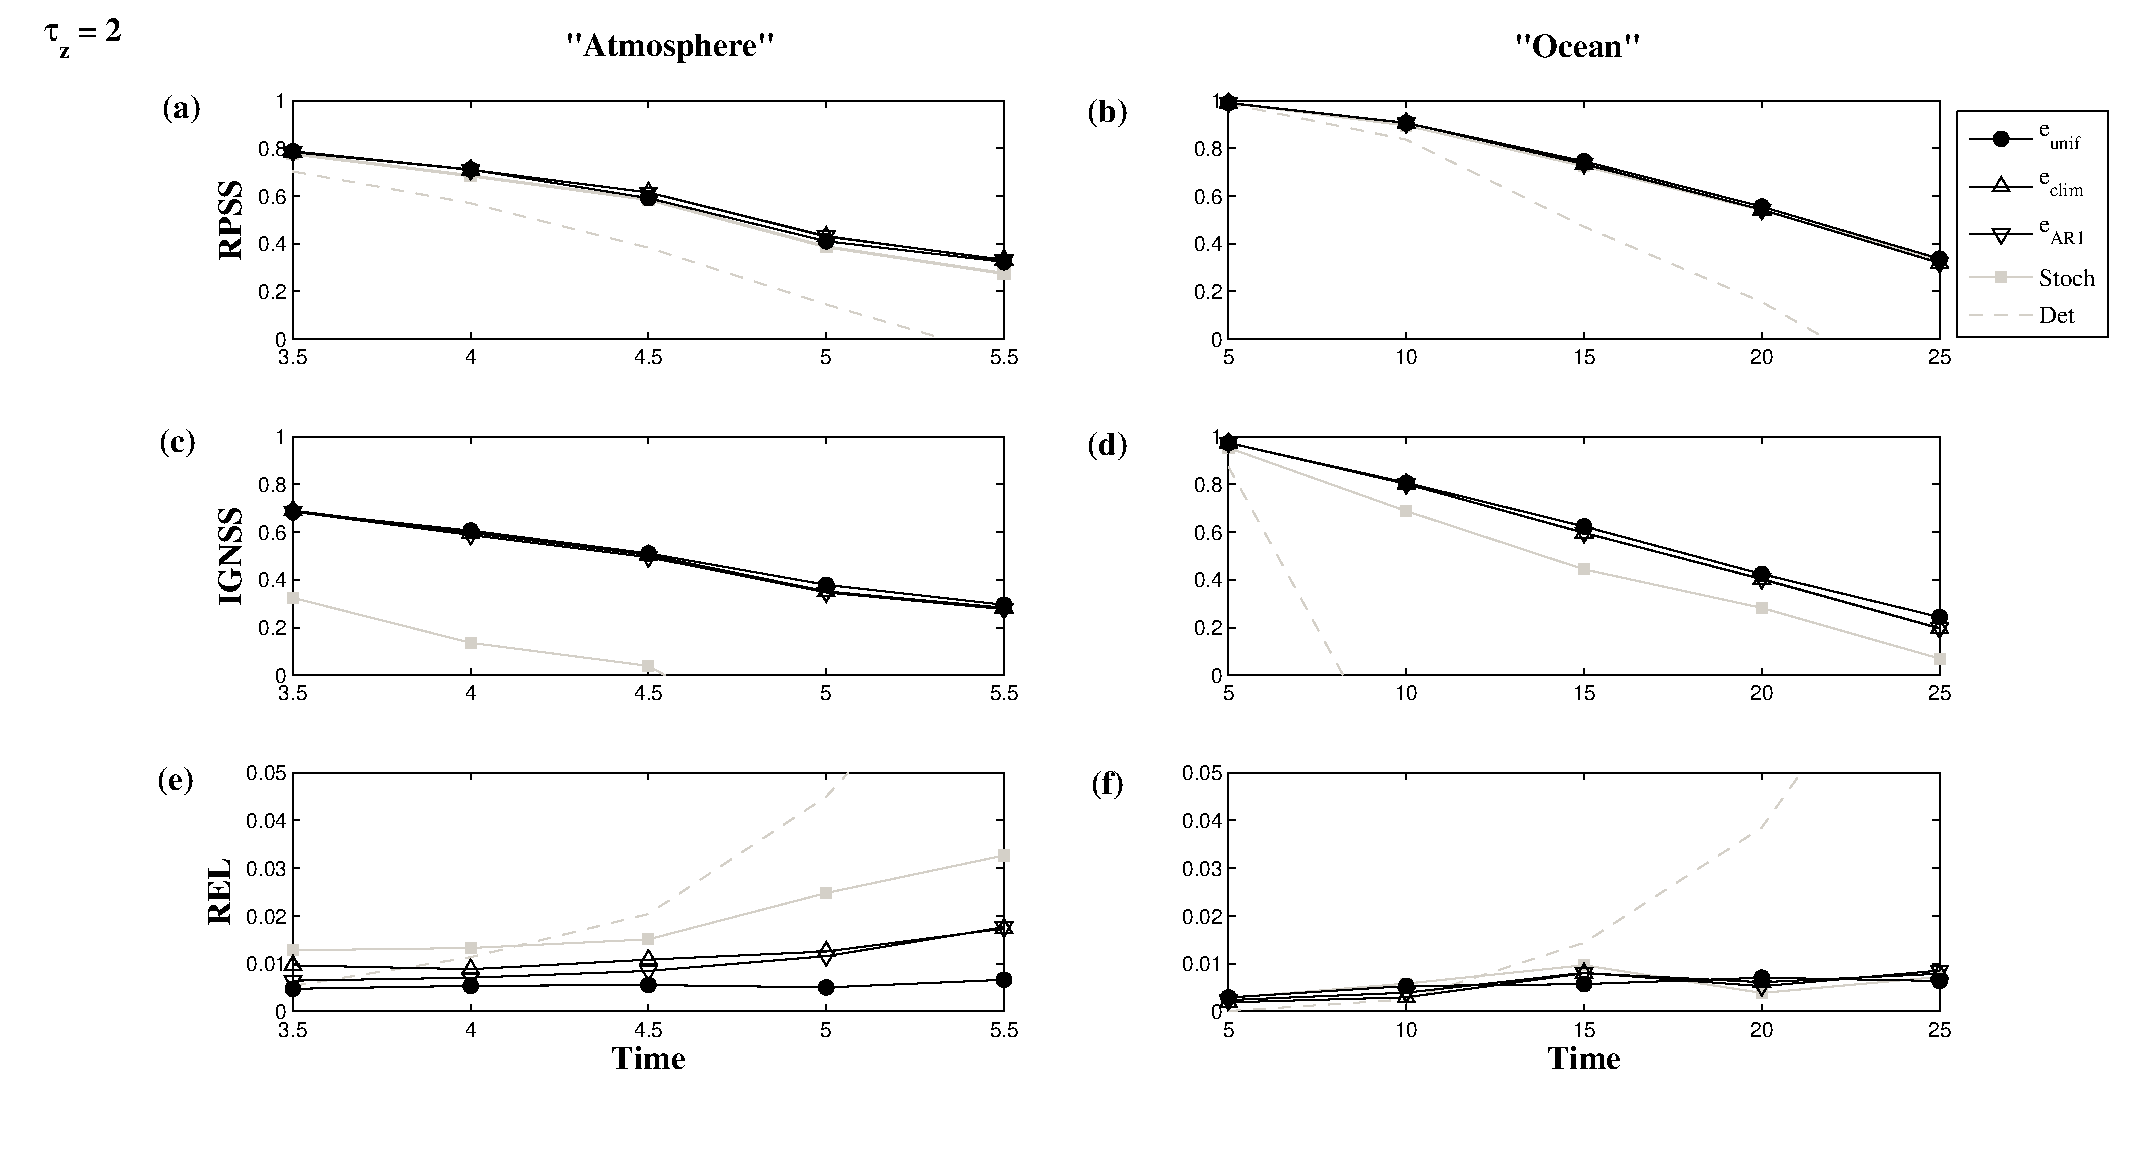
\includegraphics[width=0.5\textwidth,height=0.5\textwidth]{timeseries_alle_std00_lev8_40pt_meanao_exp1.eps}}
                \caption{\bf \label{scoreTau2}
                        Forecast scores RPSS (top), IGNSS (middle) and REL (bottom) for
                        the atmosphere (left) and ocean (right) components at $\tau_z=2$ generated by
                        $e_{\text{unif}}$ (black circle), $e_{\text{clim}}$ (black upper triangle), $e_{\text{AR1}}$ (black lower triangle),
                        \emph{Stoch} (grey square), and \emph{Det} (grey dashed-line).\
                        The PCE approximated by $64^{\text{th}}$ degree polynomial.\
                        }
        \end{figure}
        \begin{figure}[h]
                \fbox{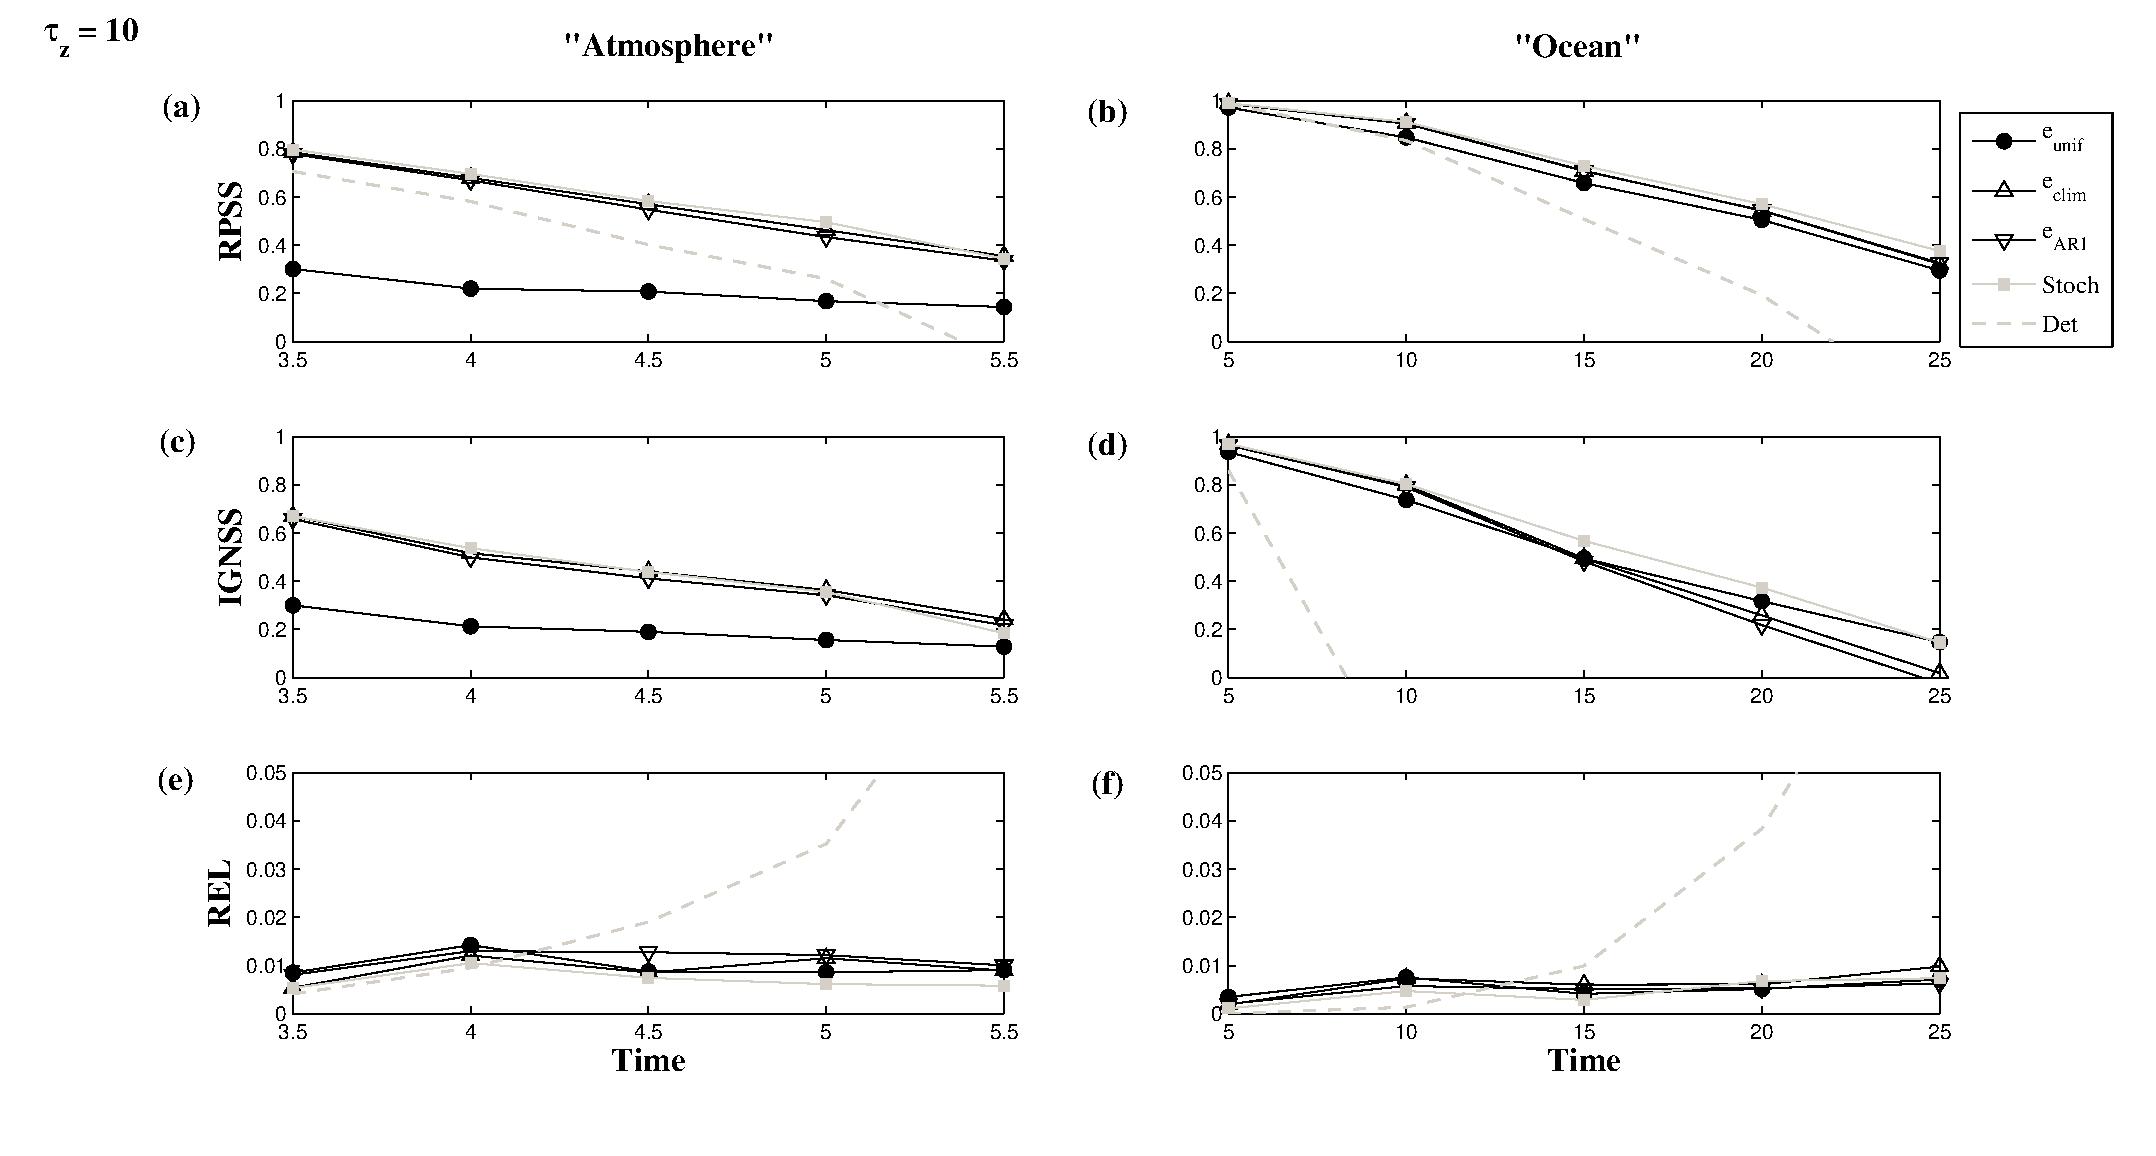
\includegraphics[width=0.5\textwidth,height=0.5\textwidth]{timeseries_alle_std00_lev8_40pt_meanao_exp2.eps}}
                \caption{\bf  \label{scoreTau10}
                        As Figure {\ref{scoreTau2}}, forecast scores RPSS, IGNSS and REL at $\tau_z=10$.\
                        }       
        \end{figure}



\end{document}
